\documentclass[sigconf,review]{acmart}

\usepackage{booktabs} % For formal tables

% Copyright
\setcopyright{none}
%\setcopyright{acmcopyright}
%\setcopyright{acmlicensed}

%\setcopyright{rightsretained}

%\setcopyright{usgov}
%\setcopyright{usgovmixed}
%\setcopyright{cagov}
%\setcopyright{cagovmixed}

%\settopmatter{printacmref=false}

%Conference
\acmConference[SCN]{Security and Communication Networks}{2018}{}

% DOI
\acmDOI{}

% ISBN
\acmISBN{}

% These commands are optional
\acmBooktitle{Security and Communication Networks}
\editor{}
\editor{}
\editor{}


\begin{document}
\title{Detection Method for Distributed Web-Crawlers: a Long-tail Threshold Model}
%\titlenote{Produces the permission block, and copyright information}

\author{Inwoo Ro}
%\orcid{1234-5678-9012}
\affiliation{%
  \institution{Dept. of Computer Science, Hanyang University}
  \city{Seoul}
  \country{Korea}
}
\affiliation{%
  \institution{NAVER WEBTOON Corp.}
  \city{Bundang}
  \country{Gyeoungi-do}
}
\email{inwoo13@hanyang.ac.kr}

\author{Joong Soo Han}
\affiliation{%
  \institution{Dept. of Computer Science, Hanyang University}
  \city{Seoul}
  \country{Korea}
}
\email{soohan@hanyang.ac.kr}

\author{Eul Gyu Im}
\orcid{0000-0002-4130-513X}
\affiliation{%
  \institution{Dept. of Computer Science, Hanyang University}
  \city{Seoul}
  \country{Korea}
  }
\email{imeg@hanyang.ac.kr}

% The default list of authors is too long for headers.
\renewcommand{\shortauthors}{I. Ro et al.}


\begin{abstract}
This paper proposes an advanced countermeasure against distributed web-crawlers. We investigated other methods for crawler detection and analyzed how distributed crawlers can bypass these methods.  Our method can detect distributed crawlers by focusing on the property that web traffics follow the power distribution. When we sort web pages by the number of requests, most of requests are concentrated on the most frequently requested web pages. In addition, there will be some web pages that normal users do not generally request. But crawlers will request for these web pages because their algorithms are intended to request iteratively by parsing web-pages to collect every items the crawlers encounter. Therefore, we can assume that if some IP addresses are frequently used to request the web pages that are located in the long-tail area of a power distribution graph, those IP addresses can be classified as crawler nodes. The experimental results with NASA web-traffic data showed that our method was effective to identify distributed crawlers with 0.0275\% false positives when a conventional frequency-based detection method shows 2.882\% false positives with an equal access threshold.
\end{abstract}


\keywords{Web Crawler, Traffic Analysis, Power Law, Information Theory}

\maketitle


%
% Introduction
%
\section{Introduction}
Web-crawling is used in various fields to collect data~\cite{r11, p2p}. Some web-crawlers collect data even though the target site prohibits crawlers by \texttt{robots.txt}. Some web services try to detect crawling activities and to prevent crawlers from accessing web pages through anti-crawler methods, but some malicious web-crawlers bypass detection methods by modifying their header values or by distributing source IP addresses to masquerade itself as if they are normal users.

Some companies prohibit web-crawlers from access their web pages because of the following reasons: First, web-crawlers may degrade the availability of web servers. Second, contents in the web servers are regarded as intellectual properties of the companies. A competing company may copy the entire data provided in a web server, and the competing company may provide similar services to clients. Even if individual data is open to be browsed by clients, crawling and collecting data from competitors can be treated as a separate issue. For example, there was a crawling lawsuit between Job Korea, Inc. and Saramin, Inc. Saramin crawled resume data from jobkorea.com, and JobKorea filed a complaint against this action. As a result, the court has imposed a fine on Saramin's crawling activities.

This paper investigates the conventional anti-crawling methods and various avoidance techniques, and shows that the conventional anti-crawling methods cannot stop distributed crawlers. Then we propose a new anti-crawling method, i.e. LTM (Long-tail Threshold Model) method which gradually adds the distributed crawlers' node IP addresses to the block-list. The experimental results showed that
our method can effectively identify distributed crawlers with
0.0275\% false positives. In the conventional frequency-based method, when the threshold is increased to detect more crawler nodes, false positives increase accordingly.

This paper is organized as follows: Section 2 describes about conventional anti-crawling methods and how distributed crawlers can bypass them.; Section 3 explains the technique of detecting distributed crawlers using the long-tail region and characteristics of the region.; In Section 4 we compare the false positive rate of the LTM with that of the conventional access frequency-based anti-crawling technique. Section 4 describes how the LTM solves this problem.; Sections 5 and 6 summarize the paper and explain future works. 

%
% Back Ground
% with 2 subsections
%
\section{Related Works}
In this section, we summarized conventional anti-crawling methods and their counter crawling measures.

\subsection{Filtering using HTTP Header information} 
A basic crawler will send requests without modification on its header information. Web servers can distinguishes a legitimate user from a crawler by checking the request header, especially if the User-Agent value has been set properly. This header checking method is a basic anti-crawling method~\cite{r10}.
However if a crawler attempts to masquerade itself as a legitimate user, it will replay with the header information from a web browser or with the HTTP header information similar to a browser. This makes it difficult for a web server to determine whether a client is a crawler or a legitimate user by simply checking the request header.

\subsection{Access Pattern-based Anti-Crawling}
An access pattern-based anti-crawling method classifies legitimate users from crawlers based on the request patterns generated by clients. If a client requests only specific web-pages continuously without calls to web-pages that should normally be requested, the client will be regarded as a crawler. A crawler performing an aggressive crawling predefines the core web-pages that the crawler wants to collect, and the crawler requests specific web-pages without requesting unnecessary web-pages. In this case, a web server can recognize that the client is not a legitimate user. With a web service that analyzes access patterns of clients, the service can distinguish crawlers from normal users based on predefined normal users' access patterns~\cite{r10}. Although this approach can recognize a crawler based on access patterns, some crawlers even masquerade their access patterns by analyzing network logs~\cite{r14}.

\subsection{Access Frequency-based Anti-Crawling}
An access frequency-based anti-crawling method determines whether a client is a crawler or a legitimate user by the access frequency threshold as the maximum number of accesses within a specific time window. If the number of requests from a client exceeds a certain threshold within the pre-defined duration, the web server classifies the client as a crawler~\cite{r14}.
This approach has two well-known problems: First, it has a vulnerability against distributed crawlers. If an attacker uses distributed crawlers such as Crawlera, the access rate of each crawler node can be managed to stay lower than the threshold. Second, there is a chance to detect normal users that share a single public IP address as a crawler.

\subsection{CAPTCHA}
CAPTCHA provides a separate test step to identify users, which must be passed first in order for users to use web services. CAPTCHA can be used to defend against crawlers but has a trade-off between security and user experience. For example, requesting additional actions from users for verification at the login phase. In addition, there is a possibility that a malicious user can reuse a session key after completing the verification normally and can execute crawlers with the session key.

%
% BLOCKING DISTRIBUTED CRAWLER
% with 2 subsections
%
\section{Blocking Distributed Crawlers}
As described in the previous section, distributed crawlers can bypass conventional anti-crawling methods. In this section, we propose a new technique to detect and to block distributed crawlers that could not be defended by conventional anti-crawling techniques.

\subsection{Required Number of Crawler Nodes}
In order for distributed crawlers to collect the entire data of a website, the following conditions must be met.

\begin{equation}
C_n \geq U_m / (T_d * 30) 
\end{equation}
where $U_m$ is the number of items updated in a month, $T_d$ is the maximum number of requests per IP address, $C_n$ is the number of crawler nodes (IP addresses) and 30 is the number of days in a month. $T_d$ multiplied by 30 was to get the number of requests per month. 

The crawler node needed to collect all the monthly updated data. The number of monthly update data was divided by the maximum number of requests per month. 
For example, if there is a web service updates $U_m$ (e.g. 30,000) items in a month and the service has a restriction rule that an IP address with more than $T_d$ (e.g. 100) requests will be blocked and an attacker who tries to collect every item from the web service will need $C_n$ (e.g. 10) crawler nodes to avoid the restriction. Therefore, as $U_m$ increases or $T_d$ decreases, $C_n$ should be increased, and $C_n$ numerically indicates the level at which the website is difficult to crawl.

\subsection{Generating Long-tail $T_d$ zones}
The number of items that are updated in a month can not be arbitrarily increased. Therefore, a simple way to prevent distributed crawlers is to decrease $T_d$, but this will also increase false positives significantly. In this paper, we solve this problem by reversing the general characteristics of web traffics and using the fact that distributed crawlers try to replicate the entire data of a web server.
If items are sorted by access rates, we can see the exponentially decreasing curve in the graph, as shown in Figure~\ref{fig:fig1}. The most the web traffics are concentrated on most frequently requested items~\cite{r3}, and there is a long-tail region that has low access rates. We calculated maximum request counts of this long-tail region and set this value as $T_{d3}$.

\begin{figure}[H]
    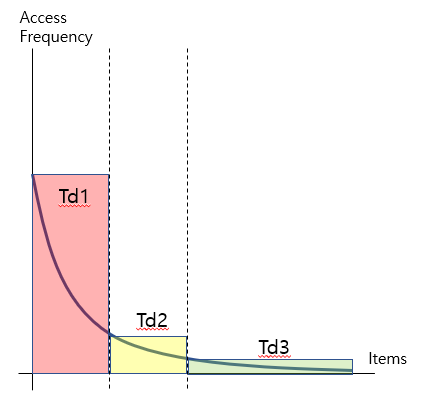
\includegraphics[width=0.7\columnwidth]{figs/figure_01.png}
    \caption{Access Frequencies per number of connections}
    \label{fig:fig1}
\end{figure}

In information theory, unlikely events are more informative than likely events, and the events in the long-tail region are more unlikely than the other events. This means that a web service can find more information from requests in the long-tail region. Hence, when a client keeps requesting items in the long-tail region, a web service can increase the count until it reaches $T_{d3}$, instead of reaching $T_d$ mean. This means that a web service can set much more sensitive threshold without increasing the false positive rate.


\subsection{Node Reducing with Long-tail Region}
In order for an attacker to collect the entire data from a web service, the attacker must also access items in the long-tail region. However, the attacker does not know exactly which items belong to the long-tail region. Using this information asymmetry, service providers can easily identify IP addresses that accessed the items more frequently than other IP addresses. These identified crawler IP addresses will be included in the block list and the number of IP addresses in the block list will be $C_m$. If we start to increase the $C_m$ value through the long-tail interval, the attacker will crawl with a smaller number of IP addresses, and $C_m$ will be increased in the $T_{d3}$ interval.

\begin{itemize}
\item $C_m$: The number of crawler nodes (IP addresses) blocked by a web service
\item long\_t: Ratio of items included in the long-tail region
\end{itemize}

So attackers must satisfy the following inequality to avoid our blocking method. $C_n$ - $C_m$ is the number of non-blocked crawler nodes and this should be greater than the right-hand side term of the following expression.

  \begin{equation}
C_n - C_m \geq (U_m * long\_t) / (T_{d3} * 30)
  \end{equation}

On the service provider side, $C_m$ should be greater than the right-hand side term to block distributed crawlers.

  \begin{equation}
C_m > C_n - (U_m * long\_t) / (T_{d3} * 30)
  \end{equation}

If a particular IP address accesses an item in the long-tail region with more than the $T_{d3}$ value determined by the above formula, it can be included in the block list.


\subsection{Dummy Items}
The service provider may add dummy items to detect crawlers, and dummy items are inaccessible from legitimate users because there are no user interfaces for dummy items or hidden. There are few ways to generate dummy items, it may exists as an HTML tag but it is not displayed on the screen by the attribute setting or it may contains a garbage information that normal users shell not be interested. But a crawler that performs sequential access to the service will may access the dummy items. By this characteristic, dummy items can work as extension of the long-tail region. In this paper, we will not include dummy items in experiments for fair comparisons with real traffic logs which do not contain any dummy items.



%
% EXPERIMENT
% 1. Web Traffic Data
% 2. Simulation
% 3. Node Reducing Result
%
\section{Experiments}
Our experiments were designed to evaluate the classification performance of our crawler detection module for web traffics. We compared our LTM (Long-tail Threshold Model) method with a normal access frequency-based anti-crawling method on the maximum number of crawler nodes and false positive rates. We used the real web traffic logs that NASA released in 1995~\cite{r15}. 

\begin{table}[H]
  \caption{Comparison of Log Data}
    \begin{tabular}{ l | l | l | l  }
    \hline
    & \# of accesses & \# of Items & \# of users \\ \hline
    $NASA$ & 1,701,011 & 7,649 & 76,040 \\ 
    $Hyderabad$ & 3,208,200 & 16 & 81,087  \\ \hline
    \end{tabular}
\label{tab:logdata}
\end{table}

Even though the web traffic logs of NASA are more than 20 years old, there are two factors why we used this dataset in our experiments. One is the number of users, and the other is the number of items in the site. The number of users is important because the traffic patterns can be biased by some users if the number of users is small. For an example,  as shown in Table~\ref{tab:logdata}, even though the Hyderabad log has a large number of accesses from a number of users, it would be difficult to build a long-tail zone for simulation since the number of items is small.

\begin{figure}[H]
    \centering
    \includegraphics[width=0.85\columnwidth]{figs/figure_02_design.png}
    \caption{Experimental Design}
    \label{fig:fig2}
\end{figure}


To accomplish this purpose, we developed a python-based data tool and a simulator. In the data preprocessing tool, raw traffic data is preprocessed as shown in Figure~\ref{fig:fig2} to count access frequencies for individual URLs and classify sets belonging to the long-tail region. The simulator determines based on preprocessed data whether the accessing node is a crawler whenever a new access occurs.

\begin{figure} [H]
    \includegraphics[width=0.88\columnwidth]{figs/figure_03_flow_chart_01.png}
    \caption{Crawler Detection Flow}
    \label{fig:fig6}
\end{figure}

\subsection{Web Traffic Data}

\subsubsection{Data Source} 

NASA released a total of 1,891,715 access logs for the month of July 1995. We parsed these logs into the \texttt{csv} format that composed of four columns including IP address, date, an access target and an access result. The total number of connected IP addresses were 81,978 and the number of items were 21,649.


\subsubsection{Data Pre-Processing and Traffic Distributions}

We performed three steps in the pre-processing phase for the experiments. The first step splits logs into two datasets: a training set and a testing set. Among NASA access logs, first 24-day logs are set as a training set and the last of logs as a testing set. The second step filters out some access logs to calculate more accurate access counts. Some requests are merged as a single request to prevent duplicated counting. For an example, when a user accesses an html file, they also get accesses to image files that are linked. This can force a multiple increase of access count. Therefore we removed some requests for image files. In addition, we excluded the request logs that the access results are not success from the experiment. After the completion of the pre-processing phase, we have a test set as shown in Table \ref{tab:preprocessing}.

\begin{table}[H]
  \caption{Pre-Processed Web Traffic Data}
    \begin{tabular}{ p{3.1cm} | p{2cm} }
    \hline
    Total Items & 7,649 \\ \hline
    Long-tail Items & 5,355 \\ \hline
    Mean of Access Counts (Total Items) & 184.76 \\ \hline
    Mean of Access Count (Long-tail Items) & 1.88 \\ \hline
    \end{tabular}
  \label{tab:preprocessing}
\end{table}

As a described in Table 1, we built a pre-processed traffic data set that consists of 7,649 items from 21,649 raw data, and it has a long-tail region that consists of 5,355 items. The mean value of total access counts was 184.76, and the mean access count of the long-tail region was 1.88. The difference between two mean values simply shows that we can set a more sensitive threshold in the crawler detection algorithm.

Table \ref{tab:expData} describes the characteristics of the most frequently accessed group ($T_{d1}$) to the least frequently accessed group ($T_{d3}$) when sorted by frequency of access. Ratio refers to the interval in which each group is located when all items are sorted by access count. For example, $T_{d2}$ is a group located between the top 0.5\% and 30\%. Mean of Access refers to the average number of accesses per item belonging to each group, and Maximum Access refers to the maximum access count among items in each group. The term Items means the number of items belonging to each group.

\begin{table}[H]
  \caption{Experiment Data}
    \begin{tabular}{ l | l | l | l | l  }
    \hline
    & Percentage & Mean of Accesses & Maximum Access & Items \\ \hline
    $T_{d1}$ &  > 0.5\% & 21,250 & 76,040 & 38 \\ 
    $T_{d2}$ & 0.5\% - 30\% & 264 & 7,043 & 2,256 \\
    $T_{d3}$ & 30\% > & 1.88 & 9 & 5,355 \\ \hline
    \end{tabular}
\label{tab:expData}
\end{table}

The key part of the experiment was to simulate the algorithm with the real web traffic data. Table~\ref{tab:expData} shows distributions of the NASA data. We checked whether the NASA data represent power distribution after sorting with access frequencies, and the traffic frequencies have power distributions as shown in Figures 2, 3 and 4.


\begin{figure}[H]
    \centering
    \includegraphics[width=0.80\columnwidth]{figs/figure_04_td1.png}
    \caption{Access Count in $T_{d1}$}
    \label{fig:fig3}
\end{figure}

Figure 3 shows the group of the most frequently requested items. 

\begin{figure}[H]
    \centering
    \includegraphics[width=0.80\columnwidth]{figs/figure_05_td2.png}
    \caption{Access Count in $T_{d2}$}
    \label{fig:fig4}
\end{figure}

\begin{figure}[H]
    \centering
    \includegraphics[width=0.80\columnwidth]{figs/figure_06_td3.png}
    \caption{Access Count in Long-tail}
    \label{fig:fig5}
\end{figure}

Figure 4 shows the long-tail region of sorted results. We set the $T_{d3}$ threshold value as 20 which is about twice larger than the maximum access rate of the long-tail region. Setting a $T_{d3}$ threshold value in LTM has a heuristic part because web services has different purposes and circumstances.

\subsection{Simulation}
In this paper, we implemented simulations for two purposes: One is to check whether LTM would be able to detect and to disable a distributed crawler IP address group and the other one is to check false positive rates when the actual web traffics are inputted to LTM. The overall crawler detection flow is shown in Figure~\ref{fig:fig6}.

\subsubsection {Distributed Crawler Detecting Simulation}

We used Python to implement the LTM simulator. The required parameters are 1) the size of the distributed IP address set used by the crawler, 2) the long-tail list, 3) the entire item list, and 4) threshold values used for detection.
When the crawler accesses an item in the long-tail region, LTM increases the access count of the source IP address. When an access count of an IP address exceeds the threshold, LTM adds the corresponding IP address to the block list. Figure 5 shows an example of running a crawler using 100 distributed IP addresses with the threshold value of 20. The long-tail ratio was 70.001\% since the number of items in the long-tail region was 5,355 while the total number of items was 7,649. Figure 7 shows a graph of the process of reducing 222 crawler sets on the simulator. 

We can observe that the crawler IP address set is gradually reduced until all the IP addresses are totally blocked. When the first crawler node IP address exceeds the $T_{d3}$ threshold and was blocked, the node reducing count increases exponentially. This is because other crawler nodes get more burden and has to access more items when a crawler node was blocked.\newline

\subsubsection{Node Reducing Result}
 
Experiments were performed with threshold set to 20, and the crawler set consisting of 222 nodes. As a result, LTM detected entire crawler nodes. False positives were about 0.0275\% which is much less than that of the conventional frequency-based crawler detection method. In Table~\ref{tab:exp1}, we compared the results of LTM with a normal FBA(frequency based anti-crawling) method.

\begin{figure}[H]
    \centering
    \includegraphics[width=0.7\columnwidth]{figs/figure_07_nr.png}
    \caption{Number of IPs reduced by detection}
    \label{fig:fig7}
\end{figure}

Detection performance of LTM against distributed crawlers can vary depending on the number of items and a long-tail ratio. Considering this limitation, simulation was conducted using old NASA traffic data(1995), total number of items were quite smaller than usual modern web services. If there is a service with 10 times data and similar access frequency distributions, our proposed method could detect distributed crawlers that consists of 2000 nodes.


\begin{table}[H]
  \caption{Experiment Data}
    \begin{tabular}{ c | r | r | r }
    \hline
    & Threshold & Max Node & False Positive \\ \hline
    LTM & 10 & 426 & 0.1239\% \\ 
    LTM & 20 & 222 & 0.0275\% \\ 
    LTM & 35 & 128 & 0.0046\% \\ 
    FBA & 10 & 573 & 8.8064\% \\
    FBA & 20 & 299 & 2.8819\% \\ 
    FBA & 35 & 173 & 0.8903\% \\ 
    FBA & 100 & 60 & 0.0367\% \\ \hline
    \end{tabular}
    \label{tab:exp1}
\end{table}

In the experiments, we compared the detection capability and the false positives between LTM and FBA with the same threshold and environments. In below graph, LIMIT\_LTM is the detection number limit of LTM with given threshold(x-axis) and LIMIT\_FRQ is the detection number limit of FBA with given threshold values.

\begin{figure}[H]
    \centering
    \includegraphics[width=0.85\columnwidth]{figs/figure_08_limit_compare.png}
    \caption{Number of Detectable Crawler Nodes}
    \label{fig:num_of_nodes}
\end{figure}

Since LTM uses the long-tail region instead of entire items, FBA detects more crawler nodes with the equivalent threshold value as shown in Figure 8. The following figures show the comparison of false positive rates of two methods. 

\begin{figure}[H]
    \centering
    \includegraphics[width=0.85\columnwidth]{figs/figure_09_fp_compare_01.png}
    \caption{False Positive: 1 to 50}
    \label{fig:fp1to50} 
\end{figure}

As we can see in Figures 9 and 10, as the threshold value in x-axis increases false positive rates and the number of detectable crawler nodes are both decreased. In the case of LTM, we can see that the false positive rates are less than 0.15\% even with the low threshold values. However, in case of FBA, the threshold value should be set to more than 76 to have similar false positive rates, which can affect the detection performance.

\begin{figure}[H]
    \centering
    \includegraphics[width=0.85\columnwidth]{figs/figure_10_fp_compare_02.png}
    \caption{False Positive: 50 to 100}
    \label{fig:FP2}
\end{figure}
 
%\begin{figure}[H]
 %   \centering
 %   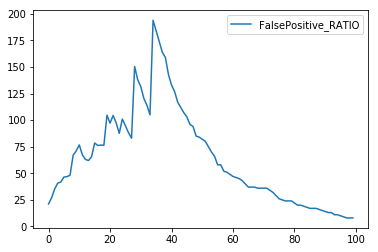
\includegraphics[width=0.85\columnwidth]{figs/figure_fp_ratio.png}
 %   \caption{Number of Detectable Crawler Nodes}
 %   \label{fig:my_label}
%\end{figure}

In the experiments, LTM reached the minimum false positive rate of 0.0046\% when FBA reached only 0.0367\%, which means that LTM has up to 500\% better detection score than the classic FBA method with the similar level of false positive rates. Even though FBA can trade off the detection score, FBA generates 798\% more false positive rates. When we set the threshold to 35 which is the value that LTM reached the minimum false positive rate, FBA generated 19,400\% more false positive rate than LTM.


%
% CONCLUSION
%
\section{CONCLUSION}
In this paper, we introduced LTM(Long-tail Threshold Model) and showed that how LTM can detect distributed crawlers effectively that other previous methods are vulnerable. By simulating with the real web traffic data, LTM effectively identified distributed crawlers and showed a significantly low level of false positive rates. Illegal web crawling against web services becomes a serious security threat. Considering that there are some crawler developer using distributed crawler proxy service~\cite{r13} for illegal purposes, LTM could improve data security of web services.


%
% FUTURE WORKS
%
\section{FUTURE WORKS}
Web traffic generally tends to generate traffic bursts at certain times~\cite{r3}. Although the experiments of this paper are based on actual traffic logs, the data used in this paper did not include any complicated cases like adding new items or traffic bursts occur with external reasons since the time period of the dataset used in the experiments contains only one-month data. However real web services should challenge with these complicated circumstances.
In order to apply the results of this paper more securely to actual services, it is necessary to study whether the item movement levels and the threshold value of long-tail area can be maintained based on actual traffic data for traffic burst occurrence cases.

\section*{Acknowledgement}
This work was partially supported by the Civil-Military Technology Cooperation Program (UM17312RD3), and was partially supported by the Human Resources program in Energy Technology (No. 20174010201170) of the Korea Institute of Energy Technology Evaluation and Planning (KETEP) grant funded by the Ministry of Trade, Industry and Energy of the Korea government.


% Bibliography
\nocite{*}
\bibliographystyle{ACM-Reference-Format}
\bibliography{exbib}


\end{document}
